%% Copernicus Publications Manuscript Preparation Template for LaTeX Submissions
%% ---------------------------------
%% This template should be used for copernicus.cls
%% The class file and some style files are bundled in the Copernicus Latex Package, which can be downloaded from the different journal webpages.
%% For further assistance please contact Copernicus Publications at: production@copernicus.org
%% https://publications.copernicus.org/for_authors/manuscript_preparation.html


%% Please use the following documentclass and journal abbreviations for preprints and final revised papers.

%% 2-column papers and preprints
\documentclass[]{article}

\usepackage{upquote,natbib,graphicx}

%% \usepackage commands included in the copernicus.cls:
%\usepackage[german, english]{babel}
%\usepackage{tabularx}
%\usepackage{cancel}
%\usepackage{multirow}
%\usepackage{supertabular}
%\usepackage{algorithmic}
%\usepackage{algorithm}
%\usepackage{amsthm}
%\usepackage{float}
%\usepackage{subfig}
%\usepackage{rotating}


\begin{document}

\title{Short communication: Inverse isochron regression for Re--Os,
  K--Ca and other chronometers}

% \Author[affil]{given_name}{surname}

\author[1]{Yang Li\\
  Institute of Geology and Geophysics, Chinese Academy of Sciences, Beijing, China\\
  and Pieter Vermeesch\\
  Department of Earth Sciences, University College London, Gower Street, London, UK
}

\maketitle

\begin{abstract}
Conventional Re--Os isochrons are based on mass spectrometric
estimates of \textsuperscript{187}Re/\textsuperscript{188}Os and
\textsuperscript{187}Os/\textsuperscript{188}Os, which often exhibit
strong error correlations that may obscure potentially important
geological complexity. Using an approach that is widely accepted in
\textsuperscript{40}Ar/\textsuperscript{39}Ar and U--Pb geochronology,
we here show that these error correlations are greatly reduced by
applying a simple change of variables, using \textsuperscript{187}Os
as a common denominator. Plotting
\textsuperscript{188}Os/\textsuperscript{187}Os
vs. \textsuperscript{187}Re/\textsuperscript{187}Os produces an
`inverse isochron', defining a binary mixing line between an inherited
Os-component whose
\textsuperscript{188}Os/\textsuperscript{187}Os-ratio is given by the
vertical intercept, and the radiogenic
\textsuperscript{187}Re/\textsuperscript{187}Os-ratio, which
corresponds to the horizontal intercept. Inverse isochrons facilitate
the identification of outliers and other sources of data dispersion.
They can also be applied to other geochronometers such as the K--Ca
method and (with less dramatic results) the Rb--Sr, Sm--Nd and Lu--Hf
methods. Conventional and inverse isochron ages are similar for
precise datasets, but may significantly diverge for imprecise ones. A
semi-synthetic data simulation indicates that, in the latter case, the
inverse isochron age is more accurate. The generalised inverse
isochron method has been added to the \texttt{IsoplotR} toolbox for
geochronology, which automatically converts conventional isochron
ratios into inverse ratios and vice versa.
\end{abstract}

%\copyrightstatement{TEXT} %% This section is optional and can be used for copyright transfers.

\section{Introduction: the conventional Re--Os isochron}  %% \introduction[modified heading if necessary]
\label{sec:intro}

The [\textsuperscript{187}Os/\textsuperscript{188}Os]-budget of a
\textsuperscript{187}Re-bearing rock or mineral can be divided into an
inherited component and a radiogenic component:
\begin{equation}
  \left[\frac{{}^{187}\mbox{Os}}{{}^{188}\mbox{Os}}\right] =
  \left[\frac{{}^{187}\mbox{Os}}{{}^{188}\mbox{Os}}\right]_{i} +
  \left[\frac{{}^{187}\mbox{Re}}{{}^{188}\mbox{Os}}\right]
  \left(\exp[\lambda_{187}t]-1\right)
  \label{eq:conventional-isochron}
\end{equation}

\noindent where $\lambda_{187}$ is the decay constant of
\textsuperscript{187}Re \citep[$= 1.666 \pm
  0.017~\mbox{yr}^{-11}$,][]{smoliar1996} and $t$ is the time elapsed
since isotopic closure. Equation~\ref{eq:conventional-isochron} forms
the equation of a line:
\begin{equation}
  y = a + b x
  \label{eq:y=a+bx}
\end{equation}

\noindent where $x =
\left[{{}^{187}\mbox{Re}}/{{}^{188}\mbox{Os}}\right]$ $y =
\left[{{}^{187}\mbox{Os}}/{{}^{188}\mbox{Os}}\right]$, $a =
\left[{{}^{187}\mbox{Os}}/{{}^{188}\mbox{Os}}\right]_i$ and $b =
\left(\exp[\lambda_{187}t]-1\right)$.  Both the independent variable
($x$) and the dependent variable ($y$) are measured quantities that
are associated with analytical uncertainty. Therefore, linear
regression of the isochron line is typically done by weighted least
squares regression with uncertainty in both variables
\citep{york2004}.

One drawback of the conventional isochron definition of
Equation~\ref{eq:conventional-isochron} is that the rarest isotope,
\textsuperscript{188}Os, which is associated with the largest mass
spectrometer uncertainties, appears in the denominator of both $x$ and
$y$. This has the potential to produce strong error correlations
\citep{stein2000}. For example, consider the following hypothetical
(independent) abundance estimates and their standard errors:
\[
X \equiv {}^{187}\mbox{Os} = 2,000 \pm 10 \mbox{~fmol;~}
Y \equiv {}^{187}\mbox{Re} = 30,000 \pm 50 \mbox{~fmol}
\mbox{~and~}
Z \equiv {}^{188}\mbox{Os} = 10 \pm 2 \mbox{~fmol}
\]

\noindent then, using the methods of \citet{pearson1896}, the ratio
correlation between [\textsuperscript{187}Os/\textsuperscript{188}Os]
and [\textsuperscript{187}Re/\textsuperscript{188}Os] is
\begin{equation}
  \noindent \rho_{\frac{X}{Z}\frac{Y}{Z}} \approx
  \frac{
    \left(\frac{s[Z]}{Z}\right)^2
  }{
    \sqrt{\left(\frac{s[Y]}{Y}\right)^2 +
      \left(\frac{s[Z]}{Z}\right)^2}
    \sqrt{\left(\frac{s[X]}{X}\right)^2 +
      \left(\frac{s[Z]}{Z}\right)^2}
  }
  =
  \frac{
    \left(\frac{2}{10}\right)^2
  }{
    \sqrt{\left(\frac{50}{30,000}\right)^2 +
      \left(\frac{2}{10}\right)^2}
    \sqrt{\left(\frac{10}{2,000}\right)^2 +
      \left(\frac{2}{10}\right)^2}
  }
  = 0.9997
  \label{eq:spurious-conventional}
\end{equation}

The strong error correlation between the two variables on the isochron
diagram is manifested as narrow and steeply inclined error ellipses,
which may graphically obscure any geologically significant trend.

As an example, consider the Re--Os dataset of \citet{morelli2007}
(Figure~\ref{fig:Morelli}a), which represents a mixture of three
samples. At first glance, this dataset appears to define an excellent
isochron with a clear slope corresponding to an isochron age of
287~Ma. However upon closer inspection, the interpretation of this fit
is not so simple:

\begin{enumerate}
\item The error ellipses exhibit a tremendous range of sizes. The plot
  is dominated by the least precise measurement (i.e. aliquot~14), and
  the remaining aliquots are barely visible.
\item The error ellipses are nearly perfectly aligned with the
  isochron, which makes it difficult to distinguish between geological
  and analytical sources of correlation.
\item The isochon fit exhibits an MSWD of 2.5, which indicates the
  presence of a moderate amount of overdispersion of the data with
  respect to the formal analytical uncertainties. It is not
  immediately clear which aliquots are responsible for the poor
  goodness-of-fit.
\end{enumerate}

\begin{figure}
  \includegraphics[height=.85\textheight]{Morelli2.pdf}
  \caption{a) conventional isochron of the Re--Os data for
    \citet{morelli2007}, with uncertainties shown as 95\% confidence
    intervals without and with $\sqrt{\mbox{MSWD}}$ overdispersion
    multiplier. b) and c) the inverse isochron diagram of the same
    data represents a mixing line between inherited and radiogenic
    components. The sample is highly radiogenic, allowing precise age
    estimation despite the presence of significant overdispersion,
    which is masked by the error correlations in the conventional
    isochron diagram. All error ellipses and confidence envelopes are
    shown at 95\% confidence.}
  \label{fig:Morelli}
\end{figure}

\section{The inverse Re--Os isochron}

All three of these problems can be solved by a simple change of
variables:
\begin{equation}
  \left[\frac{{}^{188}\mbox{Os}}{{}^{187}\mbox{Os}}\right] =
  \left[\frac{{}^{188}\mbox{Os}}{{}^{187}\mbox{Os}}\right]_i
  \left\{
    1 -
  \left[\frac{{}^{187}\mbox{Re}}{{}^{187}\mbox{Os}}\right]
  \left(\exp[\lambda_{187}t]-1\right)
  \right\}
  \label{eq:inverse-isochron}
\end{equation}

\noindent which defines an `inverse' isochron line:
\begin{equation}
  y' = a' + b' x'
  \label{eq:y'=a'+b'x'}
\end{equation}

\noindent where
$x'=\left[{{}^{187}\mbox{Re}}/{{}^{187}\mbox{Os}}\right]$,
$y'=\left[{{}^{188}\mbox{Os}}/{{}^{187}\mbox{Os}}\right]$,
$a'=\left[{{}^{188}\mbox{Os}}/{{}^{187}\mbox{Os}}\right]_i$ and
$b'=-\left[{{}^{188}\mbox{Os}}/{{}^{187}\mbox{Os}}\right]_i\left(\exp[\lambda_{187}t]-1\right)$.

Equation~\ref{eq:inverse-isochron} defines a mixing line between the
non-radiogenic
$\left[{{}^{188}\mbox{Os}}/{{}^{187}\mbox{Os}}\right]$-ratio (which
marks the vertical intercept) and the radiogenic
$\left[{{}^{187}\mbox{Re}}/{{}^{187}\mbox{Os}}\right]$-ratio (which
markes the horizontal intercept). By moving the least abundant nuclide
to the numerator of the dependent variable, instead of the denominator
of both the dependent and the independent variables, the inverse
isochron reduces the error correlations. Revisiting the earlier
hypothetical example yields an error correlation of:
\begin{equation}
  \noindent \rho_{\frac{Y}{X}\frac{Z}{X}} \approx
  \frac{
    \left(\frac{s[X]}{X}\right)^2
  }{
    \sqrt{\left(\frac{s[X]}{X}\right)^2 +
      \left(\frac{s[Y]}{Y}\right)^2}
    \sqrt{\left(\frac{s[X]}{X}\right)^2 +
      \left(\frac{s[Y]}{Y}\right)^2}
  }
  =
  \frac{
    \left(\frac{10}{2,000}\right)^2
  }{
    \sqrt{
      \left(\frac{10}{2,000}\right)^2 +
      \left(\frac{50}{30,000}\right)^2
    }
    \sqrt{
      \left(\frac{10}{2,000}\right)^2 + 
        \left(\frac{2}{10}\right)^2
    }
  }
  = 0.024
  \label{eq:spurious-inverse}
\end{equation}

Plotting the \citet{morelli2007} dataset on an inverse isochron
diagram provides a much clearer picture of it
(Figure~\ref{fig:Morelli}b and c):

\begin{enumerate}
\item Although the error ellipses still exhibit a range of sizes,
  reflecting the heteroscedasticity of the data, the imprecise
  measurements do no longer dominate the plot to the extent where they
  obscure the precise ones.
\item The error ellipses are no longer aligned parallel to the
  isochron line, but are oriented at an angle to it. This makes it
  easier to see the difference between the geological and analytical
  sources of correlation.
\item The overdispersion is clearly visible and can be attributed to
  aliquots~1, 12 and 14, whose error ellipses exhibit the smallest
  overlap with the best fit line. Most of the geochronologically
  valuable information is contained in the highly radiogenic aliquots
  7--11, which tightly cluster near the
  [\textsuperscript{187}Re/\textsuperscript{187}Os]-intercept.  Even
  though the data are overdispersed, the overall composition is very
  radiogenic and can therefore be used to obtain precise age
  constraints. The initial
  [\textsuperscript{187}Os/\textsuperscript{188}Os]-ratio, however, is
  poorly constrained.
\end{enumerate}

\section{Application to other chronometers}

Strong error correlations are commonly observed in other conventional
isochron systems, where they may arise from a number of mechanisms
including poor counting statistics (previous sections), blank
correction \citep[e.g.,][]{vermeesch2015b, connelly2017} or
fractionation \citep[e.g.,][]{ludwig1980}.  Inverse isochron ratios,
in which the radiogenic daughter isotope is used as a common
denominator, are commonplace in
\textsuperscript{40}Ar/\textsuperscript{39}Ar \citep{turner1971} and
U--Pb \citep{tera1972} geochronology. They are equally applicable to
other dating methods, such as Rb--Sr
([\textsuperscript{87}Sr/\textsuperscript{86}Sr] vs.
[\textsuperscript{87}Rb/\textsuperscript{86}Sr]), Sm--Nd
([\textsuperscript{144}Nd/\textsuperscript{143}Nd] vs.
[\textsuperscript{147}Sm/\textsuperscript{143}Nd]), Lu--Hf
([\textsuperscript{177}Hf/\textsuperscript{176}Hf] vs.
[\textsuperscript{176}Lu/\textsuperscript{176}Hf]) and K--Ca
([\textsuperscript{44}Ca/\textsuperscript{40}Ca] vs.
[\textsuperscript{40}K/\textsuperscript{40}Ca]).

In the case of K--Ca dating, the inverse approach offers similar
benefits as for the Re--Os method because \textsuperscript{44}Ca is
typically 100 times less abundant than \textsuperscript{40}Ca, thus
making the conventional isochron plot prone to strong error
correlations. Note that some K--Ca studies use \textsuperscript{42}Ca
as a normalising isotope, which is even less abundant
\textsuperscript{44}Ca, and therefore further aggravates the
problem. For other chronometers such as Rb--Sr, Sm--Nd and Lu--Hf,
whose non-radiogenic isotopes are at least as abundant as the
radiogenic daughter isotopes, the benefits of the inverse isochron
approach are less obvious.

Given a data table of conventional isochron ratios ($x$ and $y$ in
Equation~\ref{eq:y=a+bx}), it is possible to calculate the inverse
ratios ($x'$ and $y'$ in Equation~\ref{eq:y'=a'+b'x'}), their
uncertainties ($s[x']$ and $s[y']$) and error correlations
($\rho_{x'y'}$) using the following equations:
\begin{equation}
  \begin{cases}
    x' = \frac{x}{y} \\
    y' = \frac{1}{y} \\
    \left(\frac{s[x']}{x'}\right)^2 =
    \left(\frac{s[x]}{x}\right)^2 -
    2 \rho_{x,y}\left(\frac{s[x]}{x}\right)\left(\frac{s[y]}{y}\right) +
    \left(\frac{s[y]}{y}\right)^2 \\
    \left(\frac{s[y']}{y'}\right)^2 = \left(\frac{s[y]}{y}\right)^2 \\
    \rho_{x'y'} =
    \left(\frac{x'}{s[x']}\right)
    \left[
    \left(\frac{s[y]}{y}\right) -
    \rho_{xy}\left(\frac{s[x]}{x}\right)
    \right]
  \end{cases}
  \label{eq:transformation}
\end{equation}

This transformation is perfectly symmetric in the sense that it can
also be used to convert inverse isochron ratios to conventional
ones. To do this, it suffices to swap $x'$ and $y'$ for $x$ and $y$
and vice versa.

\section{A semi-synthetic test of accuracy}

\citet{dalrymple1988} assert that conventional and inverse isochron
regression are mathematically equivalent in the context of
\textsuperscript{40}Ar/\textsuperscript{39}Ar geochronology.  This is
indeed the case when the analytical uncertainties of the
parent-daughter ratios are relatively small ($<5\%$, say), as is the
case for the Re--Os example of Figure~\ref{fig:Morelli}. However, this
is no longer true when the analytical uncertainties are large, or when
the data are significantly dispersed around the best fitting isochron
line. In those cases the conventional and inverse isochrons can yield
substantially different age estimates. This is because isotopic ratios
are strictly positive quantities with skewed error distributions, and
the weighted least squares algorithm of \citet{york2004} does not take
into account this skewness.

A full theoretical discussion of this phenomenon falls outside the
scope of our short communication. Instead, we will compare and
contrast the accuracy of conventional and inverse isochrons using a
semi-synthetic dataset based on 30 K--Ca ion microprobe measurements
published by \citet{harrison2010}:

\begin{enumerate}
\item Let $x_i$ be the $i$\textsuperscript{th}
  \textsuperscript{40}K/\textsuperscript{44}Ca ratio measurement, and
  let $\sigma[x_i]$, $\sigma[y_i]$, $\rho[x_i,y_i]$ be the standard
  errors and error correlation of the corresponding
  \textsuperscript{40}K/\textsuperscript{44}Ca and
  \textsuperscript{40}Ca/\textsuperscript{44}Ca ratios.
\item Collect $n$ pairs of logratios $\{\ln[X_i],\ln[Y_i]\}$ from a
  bivariate normal distribution with means $\{\ln[x_i],\ln[y_i]\}$ and
  covariance matrix $\Sigma_i$ where
  \begin{equation}
    y_i = y_\circ + 0.895 x_i (\exp[\lambda_{40} t]-1)
    \label{eq:KCa}
  \end{equation}

  \noindent in which $y_\circ=66$ is the initial
  \textsuperscript{40}Ca/\textsuperscript{44}Ca ratio, $t=800$~Ma is
  the true K--Ca age, and
  \[
  \Sigma_i =
  \left[
    \begin{array}{@{}c@{~}c@{}}
      \frac{1}{x_i} & 0 \\
      0 & \frac{1}{y_i}
    \end{array}
    \right]
  \left[
    \begin{array}{@{}c@{~}c@{}}
      \sigma[x_i]^2 & \rho[x_i,y_i]\sigma[x_i]\sigma[y_i] \\
      \rho[x_i,y_i]\sigma[x_i]\sigma[y_i] & \sigma[x_i]^2\\
    \end{array}
    \right]
  \left[
    \begin{array}{@{}c@{~}c@{}}
      \frac{1}{x_i} & 0 \\
      0 & \frac{1}{y_i}
    \end{array}
    \right]
  \]
\item The semi-synthetic dataset is then given by $\{X_i,Y_i\}$ (for
  $1\leq{i}\leq{n}$) with covariance matrices $\Sigma'_i$ that are
  computed as follows:
  \[
  \Sigma'_i =
  \left[
    \begin{array}{@{}c@{~}c@{}}
      X_i & 0 \\
      0 & Y_i
    \end{array}
    \right]
  \Sigma_i
  \left[
    \begin{array}{@{}c@{~}c@{}}
      X_i & 0 \\
      0 & Y_i
    \end{array}
    \right]
  \]
\end{enumerate}

The logarithmic transformation is necessary to account for the
inevitable skewness of the error distributions. Even though the
semi-synthetic dataset is defined in terms of the conventional
isochron equation (Eq.~\ref{eq:KCa}), Figure~\ref{fig:Harrison} shows
that it is the inverse isochron that most accurately estimates the
age. We therefore recommend that inverse isochrons replace
conventional isochrons in Re--Os and K--Ca geochronology. The
difference between the conventional and inverse isochron age may serve
as a measure of robustness for the results.

\begin{figure}
  \includegraphics[height=.7\textwidth]{Harrison2.pdf}
  \caption{a) conventional and b) inverse isochron for a
    representative outcome of the semi-synthetic K--Ca data
    generator. The true age is 800~Ma and the true initial
    \textsuperscript{40}Ca/\textsuperscript{44}Ca ratio is 66. The
    inverse isochron better approximates these values than the
    conventional isochron. Uncertainties are shown as 95\% confidence
    intervals.}
  \label{fig:Harrison}
\end{figure}

\section{Implementation in \texttt{IsoplotR}}

Inverse isochrons have been added to all the relevant chronometers in
the \texttt{IsoplotR} toolbox for radiometric geochronology
\citep{vermeesch2018c}. This functionality can be used either from the
graphical user interface (which can be accessed both online and
offline, Figure~\ref{fig:IsoplotR}a), or from the command line, using
the \texttt{R} programming language and application programming
interface (Figure~\ref{fig:IsoplotR}b and c). \texttt{IsoplotR}
automatically executes the ratio conversion of
Equation~\ref{eq:transformation} in the background, so the user can
supply their data as conventional ratios and still plot them on an
inverse isochron diagram.

\begin{figure}[!ht]
  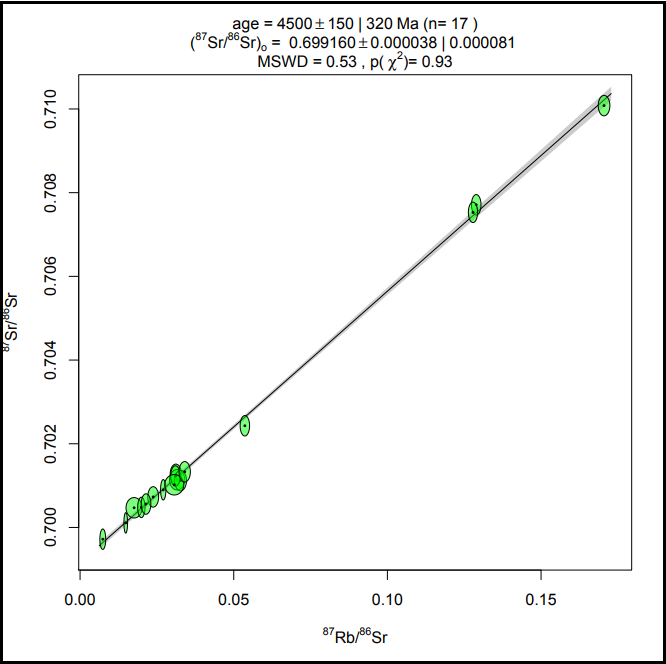
\includegraphics[width=\textwidth]{IsoplotR.pdf}
  \caption{Conventional and inverse isochrons can be constructed with
    \texttt{IsoplotR}, (a) either using its graphical user interface,
    (b--c) or from the \texttt{R} command prompt. This is illustrated
    here for a Re--Os dataset of \citet{kendall2006} that exhibits
    weaker error correlations than the example of
    Figure~\ref{fig:Morelli}. The normal (a) and inverse (c) isochron
    produce nearly identical results.}
  \label{fig:IsoplotR}
\end{figure}

\section{Conclusions}
\label{sec:conclusions}

Conventional isochrons are straight line regressions between two
ratios $D/d$ and $P/d$, where $P$ and $D$ are the parent and daughter
nuclides, and $d$ is a non-radiogenic isotope of the daughter
element. This paper reviewed the phenomenon whereby strong error
correlations arise when $d$ is less abundant than $D$, and is
therefore measured less precisely than $D$.  This is the case in
Re--Os and K--Ca geochronology, which use \textsuperscript{188}Os and
\textsuperscript{44}Ca as normalising isotopes, respectively.  These
isotopes are tens to hundreds of times less abundant than the
radiogenic \textsuperscript{187}Os and \textsuperscript{40}Ca, causing
strong error correlations. Besides this `spurious' source of
correlated uncertainties \citep[\emph{sensu}][]{pearson1896},
additional sources of covariance may include blank corrections,
calibrations and fractionation effects that apply to both variables in
the isochron regression.

The error correlation between the isochron ratio measurements can be
so strong ($r>0.99$) that it outweighs and obscures the
geochronological correlation.  This is not only inconvenient from an
esthetic point of view, but may also cause numerical problems.  It is
not uncommon for data tables to either not report error correlations
at all, or to report them to only one significant digit. However, the
difference between error correlations of $r=0.991$ and $r=0.999$, say,
may have a large effect on the isochron age. All these problems can be
solved by recasting the isochron regression into a new form, by
plotting $d/D$ vs. $P/D$.  This produces a different type of linear
trend, in which the vertical intercept yields the reciprocal daughter
ratio, and the age is not proportional to the slope of the isochron
line, but inversely proportional to its horizontal intercept.

Published datasets (which are usually tabulated in a conventional
isochron format) can be re-evaluated by transforming them to inverse
isochron ratios using Equation~\ref{eq:transformation}, either
explicitly or internally within \texttt{IsoplotR}. The two isochron
formulations produce identical results \citep{dalrymple1988} if the
relative uncertainties of the ratio measurements are reasonably small
($<5$\%, say). In the presence of larger uncertainties, inverse
isochrons produce the most accurate results. We therefore recommend
that inverse isochrons are used instead of conventional isochrons for
Re--Os and K--Ca geochronology, and any other datasets exhibiting
strong error correlations.

%% The following commands are for the statements about the availability of data sets and/or software code corresponding to the manuscript.
%% It is strongly recommended to make use of these sections in case data sets and/or software code have been part of your research the article is based on.

%\codeavailability{TEXT} %% use this section when having only software code available


%\dataavailability{TEXT} %% use this section when having only data sets available


Code and data availability: {\texttt{IsoplotR} is free software released
  under the GPL-3 license. The package and its source code are
  available from \texttt{https://cran.r-project.org/package=IsoplotR}.}\medskip

%\sampleavailability{TEXT} %% use this section when having geoscientific samples available

%\videosupplement{TEXT} %% use this section when having video supplements available

      %% use this to mark the end of the appendix section. Otherwise the figures might be numbered incorrectly (e.g. 10 instead of 1).

%% Regarding figures and tables in appendices, the following two options are possible depending on your general handling of figures and tables in the manuscript environment:

%% Option 1: If you sorted all figures and tables into the sections of the text, please also sort the appendix figures and appendix tables into the respective appendix sections.
%% They will be correctly named automatically.

%% Option 2: If you put all figures after the reference list, please insert appendix tables and figures after the normal tables and figures.
%% To rename them correctly to A1, A2, etc., please add the following commands in front of them:

%\appendixfigures  %% needs to be added in front of appendix figures

%\appendixtables   %% needs to be added in front of appendix tables

%% Please add \clearpage between each table and/or figure. Further guidelines on figures and tables can be found below.

Author contributions: {PV wrote the software and the paper. YL formulated the research question and contributed to the writing of the paper.} \medskip

Competing interests: {Pieter Vermeesch is an associate editor of \emph{Geochronology}.}\medskip

%\disclaimer{TEXT} %% optional section

\section*{Acknowledgements}

  We thank David Selby for feedback on an early version of the
  manuscript. This research was supported by National Key Research and
  Development Program of China grant \#2018YFA0702600 and National
  Natural Science Foundation of China grant \#42022022 awarded to YL;
  and by NERC standard grant \#NE/T001518/1 (`Beyond Isoplot') awarded
  to PV. Donald Davis, Ryan Ickert and an anonymous reviewer are
  thanked for their constructive reviews, which prompted us to develop
  the semi-synthetic K--Ca model.

%% REFERENCES

%% The reference list is compiled as follows:

%\bibliographystyle{copernicus}
%\bibliography{/home/pvermees/Dropbox/biblio.bib}

\begin{thebibliography}{14}
\providecommand{\natexlab}[1]{#1}
\providecommand{\url}[1]{{\tt #1}}
\providecommand{\urlprefix}{URL }
\expandafter\ifx\csname urlstyle\endcsname\relax
  \providecommand{\doi}[1]{https://doi.org/\discretionary{}{}{}#1}\else
  \providecommand{\doi}{https://doi.org/\discretionary{}{}{}\begingroup
  \urlstyle{rm}\Url}\fi

\bibitem[{Connelly et~al.(2017)Connelly, Bollard, and Bizzarro}]{connelly2017}
Connelly, J., Bollard, J., and Bizzarro, M.: {Pb--Pb chronometry and the early
  solar system}, Geochimica et Cosmochimica Acta, 201, 345--363, 2017.

\bibitem[{Dalrymple et~al.(1988)Dalrymple, Lanphere, and
  Pringle}]{dalrymple1988}
Dalrymple, G.~B., Lanphere, M.~A., and Pringle, M.~S.: {Correlation diagrams in
  $^{40}$Ar/$^{39}$Ar dating: Is there a correct choice?}, Geophysical Research
  Letters, 15, 589--591, 1988.

\bibitem[{Harrison et~al.(2010)Harrison, Heizler, McKeegan, and
  Schmitt}]{harrison2010}
Harrison, T.~M., Heizler, M.~T., McKeegan, K.~D., and Schmitt, A.~K.: {In situ
  $^{40}$K--$^{40}$Ca `double-plus' SIMS dating resolves Klokken feldspar
  $^{40}$K--$^{40}$Ar paradox}, Earth and Planetary Science Letters, 299,
  426--433, 2010.

\bibitem[{Kendall et~al.(2006)Kendall, Creaser, and Selby}]{kendall2006}
Kendall, B., Creaser, R.~A., and Selby, D.: {Re--Os geochronology of
  postglacial black shales in Australia: Constraints on the timing of
  ``Sturtian'' glaciation}, Geology, 34, 729--732, 2006.

\bibitem[{Ludwig(1980)}]{ludwig1980}
Ludwig, K.~R.: {Calculation of uncertainties of U-Pb isotope data}, Earth and
  Planetary Science Letters, 46, 212--220, 1980.

\bibitem[{Morelli et~al.(2007)Morelli, Creaser, Seltmann, Stuart, Selby, and
  Graupner}]{morelli2007}
Morelli, R., Creaser, R.~A., Seltmann, R., Stuart, F.~M., Selby, D., and
  Graupner, T.: {Age and source constraints for the giant Muruntau gold
  deposit, Uzbekistan, from coupled Re-Os-He isotopes in arsenopyrite},
  Geology, 35, 795--798, 2007.

\bibitem[{Pearson(1896)}]{pearson1896}
Pearson, K.: Mathematical contributions to the theory of evolution.--on a form
  of spurious correlation which may arise when indices are used in the
  measurement of organs, Proceedings of the Royal Society of London, 60,
  489--498, 1896.

\bibitem[{Smoliar et~al.(1996)Smoliar, Walker, and Morgan}]{smoliar1996}
Smoliar, M.~I., Walker, R.~J., and Morgan, J.~W.: {Re-Os ages of group IIA,
  IIIA, IVA, and IVB iron meteorites}, Science, 271, 1099--1102, 1996.

\bibitem[{Stein et~al.(2000)Stein, Morgan, and Scherst{\'e}n}]{stein2000}
Stein, H.~J., Morgan, J.~W., and Scherst{\'e}n, A.: {Re-Os dating of low-level
  highly radiogenic (LLHR) sulfides: The Harnas gold deposit, southwest Sweden,
  records continental-scale tectonic events}, Economic Geology, 95, 1657--1671,
  2000.

\bibitem[{Tera and Wasserburg(1972)}]{tera1972}
Tera, F. and Wasserburg, G.: {U-Th-Pb systematics in three Apollo 14 basalts
  and the problem of initial Pb in lunar rocks}, Earth and Planetary Science
  Letters, 14, 281--304, 1972.

\bibitem[{Turner(1971)}]{turner1971}
Turner, G.: {$^{40}$Ar--$^{39}$Ar ages from the lunar maria}, Earth and
  Planetary Science Letters, 11, 169--191, 1971.

\bibitem[{Vermeesch(2015)}]{vermeesch2015b}
Vermeesch, P.: {Revised error propagation of $^{40}$Ar/$^{39}$Ar data,
  including covariances}, Geochimica et Cosmochimica Acta, 171, 325--337, 2015.

\bibitem[{Vermeesch(2018)}]{vermeesch2018c}
Vermeesch, P.: {\texttt{IsoplotR}: a free and open toolbox for geochronology},
  Geoscience Frontiers, 9, 1479--1493, 2018.

\bibitem[{York et~al.(2004)York, Evensen, Mart\'{i}nez, and
  De~Basabe~Delgado}]{york2004}
York, D., Evensen, N.~M., Mart\'{i}nez, M.~L., and De~Basabe~Delgado, J.:
  {Unified equations for the slope, intercept, and standard errors of the best
  straight line}, American Journal of Physics, 72, 367--375, 2004.

\end{thebibliography}


%\begin{thebibliography}{}

%\bibitem[AUTHOR(YEAR)]{LABEL1}
%REFERENCE 1

%\bibitem[AUTHOR(YEAR)]{LABEL2}
%REFERENCE 2

%\end{thebibliography}

%% Since the Copernicus LaTeX package includes the BibTeX style file copernicus.bst,
%% authors experienced with BibTeX only have to include the following two lines:
%%
%% \bibliographystyle{copernicus}
%% \bibliography{example.bib}
%%
%% URLs and DOIs can be entered in your BibTeX file as:
%%
%% URL = {http://www.xyz.org/~jones/idx_g.htm}
%% DOI = {10.5194/xyz}


%% LITERATURE CITATIONS
%%
%% command                        & example result
%% \citet{jones90}|               & Jones et al. (1990)
%% \citep{jones90}|               & (Jones et al., 1990)
%% \citep{jones90,jones93}|       & (Jones et al., 1990, 1993)
%% \citep[p.~32]{jones90}|        & (Jones et al., 1990, p.~32)
%% \citep[e.g.,][]{jones90}|      & (e.g., Jones et al., 1990)
%% \citep[e.g.,][p.~32]{jones90}| & (e.g., Jones et al., 1990, p.~32)
%% \citeauthor{jones90}|          & Jones et al.
%% \citeyear{jones90}|            & 1990



%% FIGURES

%% When figures and tables are placed at the end of the MS (article in one-column style), please add \clearpage
%% between bibliography and first table and/or figure as well as between each table and/or figure.

% The figure files should be labelled correctly with Arabic numerals (e.g. fig01.jpg, fig02.png).


%% ONE-COLUMN FIGURES

%%f
%\begin{figure}[t]
%\includegraphics[width=8.3cm]{FILE NAME}
%\caption{TEXT}
%\end{figure}
%
%%% TWO-COLUMN FIGURES
%
%%f
%\begin{figure*}[t]
%\includegraphics[width=12cm]{FILE NAME}
%\caption{TEXT}
%\end{figure*}
%
%
%%% TABLES
%%%
%%% The different columns must be seperated with a & command and should
%%% end with \\ to identify the column brake.
%
%%% ONE-COLUMN TABLE
%
%%t
%\begin{table}[t]
%\caption{TEXT}
%\begin{tabular}{column = lcr}
%\tophline
%
%\middlehline
%
%\bottomhline
%\end{tabular}
%\belowtable{} % Table Footnotes
%\end{table}
%
%%% TWO-COLUMN TABLE
%
%%t
%\begin{table*}[t]
%\caption{TEXT}
%\begin{tabular}{column = lcr}
%\tophline
%
%\middlehline
%
%\bottomhline
%\end{tabular}
%\belowtable{} % Table Footnotes
%\end{table*}
%
%%% LANDSCAPE TABLE
%
%%t
%\begin{sidewaystable*}[t]
%\caption{TEXT}
%\begin{tabular}{column = lcr}
%\tophline
%
%\middlehline
%
%\bottomhline
%\end{tabular}
%\belowtable{} % Table Footnotes
%\end{sidewaystable*}
%
%
%%% MATHEMATICAL EXPRESSIONS
%
%%% All papers typeset by Copernicus Publications follow the math typesetting regulations
%%% given by the IUPAC Green Book (IUPAC: Quantities, Units and Symbols in Physical Chemistry,
%%% 2nd Edn., Blackwell Science, available at: http://old.iupac.org/publications/books/gbook/green_book_2ed.pdf, 1993).
%%%
%%% Physical quantities/variables are typeset in italic font (t for time, T for Temperature)
%%% Indices which are not defined are typeset in italic font (x, y, z, a, b, c)
%%% Items/objects which are defined are typeset in roman font (Car A, Car B)
%%% Descriptions/specifications which are defined by itself are typeset in roman font (abs, rel, ref, tot, net, ice)
%%% Abbreviations from 2 letters are typeset in roman font (RH, LAI)
%%% Vectors are identified in bold italic font using \vec{x}
%%% Matrices are identified in bold roman font
%%% Multiplication signs are typeset using the LaTeX commands \times (for vector products, grids, and exponential notations) or \cdot
%%% The character * should not be applied as mutliplication sign
%
%
%%% EQUATIONS
%
%%% Single-row equation
%
%\begin{equation}
%
%\end{equation}
%
%%% Multiline equation
%
%\begin{align}
%& 3 + 5 = 8\\
%& 3 + 5 = 8\\
%& 3 + 5 = 8
%\end{align}
%
%
%%% MATRICES
%
%\begin{matrix}
%x & y & z\\
%x & y & z\\
%x & y & z\\
%\end{matrix}
%
%
%%% ALGORITHM
%
%\begin{algorithm}
%\caption{...}
%\label{a1}
%\begin{algorithmic}
%...
%\end{algorithmic}
%\end{algorithm}
%
%
%%% CHEMICAL FORMULAS AND REACTIONS
%
%%% For formulas embedded in the text, please use \chem{}
%
%%% The reaction environment creates labels including the letter R, i.e. (R1), (R2), etc.
%
%\begin{reaction}
%%% \rightarrow should be used for normal (one-way) chemical reactions
%%% \rightleftharpoons should be used for equilibria
%%% \leftrightarrow should be used for resonance structures
%\end{reaction}
%
%
%%% PHYSICAL UNITS
%%%
%%% Please use \unit{} and apply the exponential notation

\end{document}
